\documentclass[10pt]{article}
% \usepackage[margin=1in]{geometry}
% \newcommand\hmmax{0}
% \newcommand\bmmax{0}
% % % Fonts% %
\usepackage{luatexja}

\usepackage[T1]{fontenc}
   % \usepackage{textcomp}
   % \usepackage{newtxtext}
   % \renewcommand\rmdefault{Pym} %\usepackage{mathptmx} %\usepackage{times}
\usepackage[complete, subscriptcorrection, slantedGreek, mtpfrak, mtpbb, mtpcal]{mtpro2}
   \usepackage{bm}% Access to bold math symbols
   % \usepackage[onlytext]{MinionPro}
   \usepackage[no-math]{fontspec}
   \defaultfontfeatures{Ligatures=TeX,Numbers={Proportional}}
   \newfontfeature{Microtype}{protrusion=default;expansion=default;}
   \setmainfont[Ligatures=TeX]{Source Serif Pro}
   \setsansfont[Microtype,Scale=MatchLowercase,Ligatures=TeX,BoldFont={* Semibold}]{Source Sans Pro}
   \setmonofont[Scale=0.8]{Atlas Typewriter}
   % \usepackage{selnolig}% For suppressing certain typographic ligatures automatically
   \usepackage{microtype}
% % % % % % %
\usepackage{amsthm}         % (in part) For the defined environments
\usepackage{mathtools}      % Improves  on amsmaths/mtpro2
\usepackage{amsthm}         % (in part) For the defined environments
\usepackage{mathtools}      % Improves on amsmaths/mtpro2
\usepackage{xfrac}

% % % The bibliography % % %
\usepackage[backend=biber,
  style=authoryear-comp,
  bibstyle=authoryear,
  citestyle=authoryear-comp,
  uniquename=false,
  % allinit,
  % giveninits=true,
  backref=false,
  hyperref=true,
  url=false,
  isbn=false,
  useprefix=true,
  ]{biblatex}
\DeclareFieldFormat{postnote}{#1}
\DeclareFieldFormat{multipostnote}{#1}
% \setlength\bibitemsep{1.5\itemsep}
\newcommand{\noopsort}[1]{}
\addbibresource{Thesis.bib}

% % % % % % % % % % % % % % %

\usepackage[inline]{enumitem}
\setlist[enumerate]{noitemsep}
\setlist[description]{style=unboxed,leftmargin=\parindent,labelindent=\parindent,font=\normalfont\space}
\setlist[enumerate]{noitemsep}

% % % Misc packages % % %
\usepackage{setspace}
% \usepackage{refcheck} % Can be used for checking references
% \usepackage{lineno}   % For line numbers
% \usepackage{hyphenat} % For \hyp{} hyphenation command, and general hyphenation stuff
\usepackage{subcaption}
% % % % % % % % % % % % %

% % % Red Math % % %
\usepackage[usenames, dvipsnames]{xcolor}
% \usepackage{everysel}
% \EverySelectfont{\color{black}}
% \everymath{\color{red}}
% \everydisplay{\color{black}}
\definecolor{fuchsia}{HTML}{FE4164}%Neon Fuchsia %{F535AA}%Neon Pink
% % % % % % % % % %

\usepackage{pifont}
\newcommand{\hand}{\ding{43}}
\usepackage{array}


\usepackage{multirow}
\usepackage{adjustbox}

\usepackage{titlesec}

\usepackage{multicol}

\setcounter{secnumdepth}{4}
\setcounter{tocdepth}{4}

\usepackage{tikz}
\usetikzlibrary{bending,arrows,positioning,calc}
\usetikzlibrary{arrows.meta}
\usepackage{tikz-qtree} %for simple tree syntax
% \usepgflibrary{arrows} %for arrow endings
% \usetikzlibrary{positioning,shapes.multipart} %for structured nodes
\usetikzlibrary{tikzmark}
\usetikzlibrary{patterns}


\usepackage{graphicx} % for images (png/jpeg etc.)
\usepackage{caption} % for \caption* command


\usepackage{tabularx}

\usepackage{bussalt}

\usepackage{Oblique} % Custom package for oblique commands
\usepackage{CustomTheorems}

\usepackage{svg}
\usepackage[off]{svg-extract}
\svgsetup{clean=true}

\usepackage{dashrule}

\newcommand{\hozline}[0]{%
  \noindent\hdashrule[0.5ex][c]{\textwidth}{.1pt}{}
  %\vspace{-10pt}
  % \noindent\rule{\textwidth}{.1pt}
}

\newcommand{\hozlinedash}[0]{%
  \noindent\hdashrule[0.5ex][c]{\textwidth}{.1pt}{2.5pt}
  %\vspace{-10pt}
}

\usepackage{contour}
% \usepackage{pdfrender}

\usepackage{extarrows}

% % % My commands % % %
\newcommand{\future}[1]{\ensuremath{\mathcal{#1}}}
\newcommand{\futpro}{\ensuremath{\mathcal{p}}}
\newcommand{\futin}{\ensuremath{\Sigma}}
\newcommand{\futout}{\ensuremath{\chi}}
% % % % % % % % % % % %

\usepackage[hidelinks,breaklinks]{hyperref}

\title{Asynchronous effects}
\author{Ben Sparkes}
% \date{ }


\begin{document}

\maketitle


\section{Introduction}
\label{sec:introduction}


\begin{itemize}
\item Main feature of cases of interest:
  \begin{enumerate}
  \item An agent is confident that some piece of reasoning would demonstrate that a particular conclusion follows from some support.
  \end{enumerate}
\item Three additional features.
  \begin{enumerate}[resume]
  \item Agent is confident that the support holds.
  \item The agent is confident that they (the agent) are able to reason from the support to the conclusion.
    \begin{itemize}
    \item Though, note somewhere (maybe here) that the agent may be assisted in this reasoning.
    \end{itemize}
  \item And, the agent adopts an attitude toward the conclusion on the basis of the prior features.
  \end{enumerate}
\item Term this \emph{speculation.}\nolinebreak
  \footnote{Something about how the term is used, esp.\ in CS.}
\item Goal is to provide a framework for thinking about a certain type of scenario which falls under this general description.
\item Central case: Morse \& Lewis.
\end{itemize}

\begin{scenario}
  More and Lewis are police officers.
  The pair have been working together for some time, and each consider st the other an equal (in their role as a police officer).
  The equality is supported their experience working together, and reflected in their working methodology:
  Any part of an investigation may be worked on by either Morse or Lewis, and no type of work has been done exclusively by either.
  Morse is confident that they could do any work Lewis does, and likewise Lewis is confident that they could do any work that Morse does.

  The pair are working on an investigation and share a casebook containing all the evidence they have gather so far.
  Lewis returns home from their day off to discover a message from Morse on their answering machine.
  Morse says, in so few words, that they, in the absence of any new evidence, have been reviewing the casebook and what evidence they do have supports bringing in Woodthorpe for questioning.
  Morse is not loquacious, and Morse does not explain their reasoning in the message.
  Lewis listens to the message and goes to bed.

  The following morning, and to Lewis' surprise, Lewis spots Woodthorpe on their way to the police station.
  And, Given Morse's message, Lewis arrests Woodthorpe.
\end{scenario}

\begin{enumerate}
\item Lewis is confident that there is some piece of reasoning would demonstrate that Woodthorpe's arrest is supported by the evidence contained in the case book.
\item Lewis is confident that the contents of the casebook constitute evidence.
\item Lewis is confident that both they and Morse are able to reason to the support for Woodthorpe's arrest from the casebook.
\item Lewis adopted some attitude to the proposition that Woodthorpe being arrested, and the action of arresting Woodthorpe (in part) depended on Lewis forming that attitude.
\end{enumerate}

\begin{itemize}
\item In ideal case, Lewis would have done the reasoning.
\item Indeed, in the ideal case Lewis would not be unaware of what follows from their evidence.
\end{itemize}

\begin{itemize}
\item Other explanations are possible, discuss some of these in what follows.
\item Two things to note:
  \begin{itemize}
  \item Lewis has confidence of the possibility of reasoning, and on this basis forms an attitude an arrests.
    \begin{itemize}
    \item Could think that Lewis straightforwardly forms an attitude toward the proposition, understands Morse as providing testimony, of a sort.
    \item There may be good reason to make this move, but it comes with some difficulties.
      \begin{enumerate}
      \item Morse didn't explicitly provide testimony.
      \item Can add some complexity to the case, assume that there are some claims in the dossier that only Lewis is aware of the evidence for, and hence Morse is restricted to only making a claim about what follows.
      \end{enumerate}
    \item Bracket testimony for the paper.
    \item Confidence is key, and while this may be supported by testimony, it is not necessary.
      The equality and history establish this without directly appealing to testimony.
    \end{itemize}
  \item It is important that Lewis is able to follow the support for the arrest.
    \begin{itemize}
    \item There are many ways to explain why this would be important for Lewis, and there are many ways to explain why this would not be important for Lewis.
    \item Sometimes this may not matter for the agent.
      \begin{itemize}
      \item If Morse is expected to do the heavy lifting, then perhaps Lewis only needs to understand that there is reason for arresting Woodthorpe.
      \item Lewis doesn't really care.
      \end{itemize}
    \item However, assume that it is important here.
      \begin{itemize}
      \item Can assume that Lewis would not arrest if there wasn't evidence.
      \item Lewis is aware that they themselves will need to justify the arrest.
      \item Lewis expects to fully understand the case file, etc.\
      \end{itemize}
    \end{itemize}
  \end{itemize}
\item Mention issue of justification, and that there's some things that can be read into the scenario that go a little beyond the basics that I'll be focusing on to start with.
\end{itemize}

\begin{itemize}
\item More can be said about the details.
\item For now, turn to an broad characterisation.
\item Goal is to provide an abstract account of the main features, allowing us to reason about the general features of these types of cases.
\item Framework!
\end{itemize}


\newpage



Reasoning is understood as process which moves from some input to some output.
The reasoning is whatever that processes is, independent of any description of it.

Example:

\(2 + 2 = 4\)
\(f(2,2) = 4\)
\(2 \Rightarrow 10, 2\Rightarrow 10 \rightarrow 100 \Rightarrow 4\)
And then there's the instantiation of this.

To keep this type distinction, talk about processes and functions.

propositional and doxastic justification to help capture the difference.



\newpage


\section{Framework}
\label{sec:framework-1}

\subsection{Reasoning}
\label{sec:reasoning}

\begin{itemize}
\item Function
\item Algorithm
\item Process
\end{itemize}

Function states the ins and out.
Algorithm details how the function works.
\begin{itemize}
\item The details can vary.
\item Example with addition, maybe.
  \begin{itemize}
  \item \(2 + 2 = 4\) tells us a little about the way in which \(4\) was obtained from \(2\) and \(2\).
    This is different from \(2 \times 2 = 4\), and different from \(2^{2} = 4\), etc.
    However, it doesn't go into detail on how addition was made.
    Can specify this in some more detail, etc.\
  \end{itemize}
\end{itemize}
Process witnesses/instantiates the function/algorithm.

\begin{itemize}
\item This is a simple view, and things can get messy.
  Especially if dealing with non-monotonic or ecological reasoning, where there may be no easy way to 
\end{itemize}


\begin{itemize}
\item This is an explicit representation, and allows functions, algorithms, and processes to all be distinct entities.
  \[\exists f \exists a \exists p \exists S \exists c(fS = c \land f \multimap p \land f \triangleright a)\]
\item Can ignore certain elements, such as the algorithm.
  \[\exists f \exists p(f\futin = \futout \land f \multimap p)\]
\item If the algorithm is ignored, can think of the process as implicitly specifying the function, and hence could simplify.
  \[\exists p(p\futin = \futout)\]
  \begin{itemize}
  \item Possible to introduce additional notation to directly link processes and algorithms here.
  \end{itemize}
\item Likewise, may assume that a function of the relevant kind is always witnessed by some process, and so adopt:
  \[\exists f(f\futin = \futout)\]
\item Here, can put algorithm back in.
  \[\exists f \exists a(f\futin = \futout \land f \triangleright a)\]
\item For simplicity, adopt the assumption that functions of the appropriate kind are witnessed by processes, and same for algorithms.
\item I have nothing interesting to say about how the process of reasoning works.
\item And, most of the time not too interested in the algorithm, so focus on:
  \[\exists f(f\futin = \futout)\]
\end{itemize}

\begin{itemize}
\item Lewis is confident \emph{that} \[\exists f(f\futin = \futout)\]
\end{itemize}



\begin{itemize}
\item Two different types of reasoning, briefly characterised.
\end{itemize}

\begin{itemize}
\item Incorporeal:
  \begin{itemize}
  \item Lewis does some reasoning on the basis of there existing some reasoning which demonstrates the support for arresting Woodthorpe.
  \end{itemize}
\item Speculative:
  \begin{itemize}
  \item Lewis takes there to be support for arresting Woodthorpe on the basis of reasoning that Lewis hasn't yet done.
  \end{itemize}
\end{itemize}

\begin{figure}[h]
  \begin{subfigure}{.5\textwidth}
    \centering
    \begin{tikzpicture}[
      ->,
      >=stealth',
      % auto,
      node distance=0cm, every text node part/.style={align=center},
      ]

      \node [] (c) at (0,0) {};
      \node [] (d) at (-3,0) {};
      \node [] (e) at (3,0) {};
      \node [] (f) at (0,-2.1) {};

      \node (1) at (0,-.1) {\(\{\exists f (f\futin = \futout)\} \cup \futin\)};
      \node (2) at (0,-2) {\(\futout\)};

      \draw [->] (1.270) to [] node[left] {\(g\)} (2.90);
    \end{tikzpicture}
    \caption{Incorporeal \\ Gather up the resources along with the existential.}
    \label{fig:non-constructive}
  \end{subfigure}
  % \hfill
  \begin{subfigure}{.5\textwidth}
    \centering
    \begin{tikzpicture}[
      ->,
      >=stealth',
  % auto,
      node distance=0cm, every text node part/.style={align=center},
      ]

      \node [] (c) at (0,0) {};
      \node [] (d) at (-3,0) {};
      \node [] (e) at (3,0) {};
      \node [] (f) at (0,-2.1) {};

      \node (1) at (0,-.1) {\(\futin\)};
      \node (2) at (0,-2) {\(\futout\)};

      \node (x) at (-2,-1.05) {\(\exists f(f\futin = \futout)\)};

      \draw [->] (1.270) to [] node[left] (3) {\(\future{f}\)} (2.90);

      \node (4) [left of=3, xshift=-2cm] {}; % {\(\exists f (f\Phi = \psi)\)};
      \draw [-{Circle[open]}] (x.0) to node[below] {\(l\)} (3.180);

    \end{tikzpicture}
    \caption{Speculative \\ Use the existential to secure a promise of a witness.}
    \label{fig:speculative}
  \end{subfigure}
\end{figure}

\begin{note}
  It seems as though there are cases where the distinction between witnessing the process and witnessing the algorithm may matter.
  For example, you inform my that you're reasoning from \(\futin\) to \(\futout\), but your reasoning was quite detailed.
  I may be confident that \(\futin\), and so form an attitude to \(\futout\).
  However, what matters to me is that your reasoning was adequate, not that I do the reasoning.
  Hence, I check your reasoning, but I do this in a piecemeal way, so I never instantiate the algorithm itself, but having verified that the algorithm works, I'm satisfied that my attitude toward \(\futout\) is adequately supported.
  \begin{itemize}
  \item Still, these types of cases can still be understood in terms of the simplified formalism.
  \end{itemize}
\end{note}








\newpage


\section{Basic Idea}
\label{sec:basic-idea}

An agent reasoning from some body of information \(\Phi\) to a proposition \(\psi\) is a process.
Abstracting away from the details of how the agent reasons from \(\Phi\) to \(\psi\), the process can be though of as an application of some function \(f\) such that \(f(\Phi) = \psi\).

% In simple cases an agent may perceive their reasoning as the result of a simple, single, process.
% For example, an agent may represent the addition of two numbers.
% However, in many cases an agent reasoning from some body of information to a proposition may be the result of composing many distinct processes, some of which can be seen as reasoning from some part of the body of information to intermediate propositions which are in turn used in additional processes to reach the proposition that concludes the agent's reasoning.
% Syntactic derivations in a first-order proof system provides a model of how agents may reason about truth-functional statements describing a domain of individuals, where rules such as conjunction introduction or universal elimination identify simple processes that can be composed to provide a proof.
% Whether or not any given first-order proof system provides an accurate, useful, information, and so on \dots, model of certain kinds of truth function statements can be questioned.
% And, whether or not an agent's reasoning from \(\{Pa \land Pb \rightarrow Qc, Pa, Pb\}\) to  \(Qc\) is a single process involving a generalised form of \emph{modus ponens} or the combination of conjunction introduction and conditional elimination may have no clear answer.
% Even so, to the extent that reasoning is the process of transforming some input to some output we can abstract from the details of what the process involves a speak of the inputs and outputs of some function.

In many cases \emph{that} \(f(\Phi) = \psi\) is novel information.
Most may have memorised that \(2 + 2 = 4\), but that \(1204 + 256 = 1280\) is a discovery made with some effort.
Some may go on to memorise that \(1204 + 256 = 1280\) and hence avoid the effort of discovering the result of adding \(1024\) and \(256\) again and would cite their initial reasoning to support their appeal to the equality in future instances of reasoning.
Others may quickly forget and rediscover the result of adding \(1024\) and \(256\) as needed.
Still, that a some instance of reasoning establishes a winning strategy for a game of chess, that the contents of a dossier demonstrates an individuals guilt, or that purchasing starfruit is a means to an end is typically novel information.

Our interest is in cases where an agent comes to be confident that some reasoning from a body of information would establish a certain proposition.
Abstractly, the agent comes to be confident that there exists some process \(f\) such that \(f(\Phi) = \psi\); the agent is confident that \(\exists f(f(\Phi) = \psi)\).
More specifically, the agent comes to be confident that they themselves are able to reason from \(\Phi\) to \(\psi\) by some process.
Hence, the agent is not only confident that some reasoning can be done; the agent is also confident that they can do the reasoning.



\begin{figure}[h]
  \begin{subfigure}{.5\textwidth}
    \centering
    \begin{tikzpicture}[
      ->,
      >=stealth',
      % auto,
      node distance=0cm, every text node part/.style={align=center},
      ]

      \node [] (c) at (0,0) {};
      \node [] (d) at (-3,0) {};
      \node [] (e) at (3,0) {};
      \node [] (f) at (0,-2.1) {};

      \node (1) at (0,-.1) {\(\{\exists f (f\futin = \futout)\} \cup \futin\)};
      \node (2) at (0,-2) {\(\futout\)};

      \draw [->] (1.270) to [] node[left] {\(g\)} (2.90);
    \end{tikzpicture}
    \caption{Incorporeal \\ Gather up the resources along with the existential.}
    \label{fig:non-constructive}
  \end{subfigure}
  % \hfill
  \begin{subfigure}{.5\textwidth}
    \centering
    \begin{tikzpicture}[
      ->,
      >=stealth',
  % auto,
      node distance=0cm, every text node part/.style={align=center},
      ]

      \node [] (c) at (0,0) {};
      \node [] (d) at (-3,0) {};
      \node [] (e) at (3,0) {};
      \node [] (f) at (0,-2.1) {};

      \node (1) at (0,-.1) {\(\futin\)};
      \node (2) at (0,-2) {\(\futout\)};

      \node (x) at (-2,-1.05) {\(\exists f(f\futin = \futout)\)};

      \draw [->] (1.270) to [] node[left] (3) {\(\future{f}\)} (2.90);

      \node (4) [left of=3, xshift=-2cm] {}; % {\(\exists f (f\Phi = \psi)\)};
      \draw [-{Circle[open]}] (x.0) to [] (3.180);

    \end{tikzpicture}
    \caption{Speculative \\ Use the existential to secure a promise of a witness.}
    \label{fig:speculative}
  \end{subfigure}
\end{figure}

\begin{note}
  The key difference between the two patterns of reasoning is the use of the guarantee that there is some way to reason from \(\Phi\) to \(\psi\).
\end{note}


\section*{Structure}
\label{sec:structure}


\begin{enumerate}
\item Start with a brief explanation of what's going on.
  \begin{enumerate}
  \item Thinking in terms of functions.
    \begin{enumerate}
    \item Functions describing processes, not committal on metaphysical type, but concrete.
    \item Contrast to mathematics case where there's some function to calculate a result.
      \begin{enumerate}
      \item In the cases I'm thinking of, the agent could be confident about what that function is, but this still leaves the particular reasoning unfulfilled.
      \end{enumerate}
    \end{enumerate}
  \end{enumerate}
\item Initial demonstration with Morse and Lewis.
  \begin{enumerate}
  \item Here, Morse provides information and Lewis goes on to arrest the suspect.
  \item Some arguments to make the structure more plausible.
  \item Three different kinds of reasoning.
  \item Speculation, as the case I'm interested in.
    \begin{enumerate}
    \item Important feature that some further use is made of the promise, the promise is expected to be fulfilled.
    \item No clear normative intuitions and complexity.
    \end{enumerate}
  \end{enumerate}
\end{enumerate}

\section{Introduction}
\label{sec:introduction}

\begin{note}
  Identify and provide a framework.
  Intuitively, some instances are permissible and others impermissible.
  Will not make any strong normative claims, and instead sketch how the framework can be used to make an argument.
  (Basically, in the superman case no way to fulfil promise, while in the taxes case there is.)
\end{note}


So, I think there's something of interest here because one often assumes that the link is what reasoning is.
An individual could not arrive at the conclusion if they did not reason from the premises.
If this is the case, then the companion is essential, as it is the companion that provides the link.
However, in many respects the companion is not essential, and the attitude has all the properties one would associate with the attitude if it had been reasoned to.
The agent may not have established the attitude in the way we would wish an ideal agent to, but we're not ideal agents.

For sure, if the agent can go through the companion, then there's nothing interesting.
This doesn't seem to be the case, however.

The real interest is in this idea of promises, and asynchronous agency.
Promises are a semi-formal construction.
So termed due to features of mundane promises, and connexion to computer science.

The key is that there's really nothing substantive about the idea of a promise.
It is, more-or-less a structural idea.



\section{Chess}
\label{sec:chess}

\begin{scenario}[Chess]\label{scen:chess}
  An agent and a companion are playing chess.
  Multiple games of chess, in fact.
  Truthfully, the agent and companion are playing as many games of chess as you would like them to play.

  Both the agent and companion want to win each game played.
  Both have a clear view of the board on any given turn, and both grasp the rules of chess.
  Still, both the agent and the companion are \emph{bounded} --- it takes time and for effort for reach to reason through potential moves and strategies.

  Communication between the agent and companion is restricted.
  By mutual agreement each is only allowed to ask their opponent if their is a winning strategy for a certain player, and the opponent is only allowed to respond `yes', `no', and `maybe'.
  If a player is truthful, then `yes' indicates a winning strategy exists for the stated player, `no' indicates a winning strategy exists for the unstated player, and `maybe' indicates the player has no been able to determine whether a winning strategy exists.

  Every time the agent has settled on an answer to whether a winning strategy for a player exists and then asked the companion whether a winning strategy for the player exists, the companion has responded with the same answer that the agent would give if the agent were to answer truthfully.
  For example, if the agent has discovered a winning strategy for the player the companion has responded `yes', and if the agent has been unable to discover a winning strategy the companion has responded `maybe'.

  Given that the companion's response to a question of whether a winning strategy exists has always coincided with the truthful response that an agent would provide to the same question, the agent is confident that they and the companion are equally matched with respect to discovering winning strategies.

  It is unlikely that that the agent's confidence rests on a single game.
  For, if the companion provides a response at random then there is a one in three chance that the companion's response matches the truthful response an agent would provide.
  However, you have as many games as you would like to grant the agent confidence that the agent and the companion are equally matched with respect to discovering winning strategies.

  Perhaps more games follow, but now confidence has been granted something unexpected happens.
  The agent looks at the board and given the agent's past experience and the arrangement of the remaining pieces, the agent is confident that they are able to settle on whether or not a winning strategy exists for their opponents.
  Yet, before the agent settles on yes or no, they ask the companion whether a winning strategy exists for the companion.
  The companion answers `yes'.

  \begin{note}
    These responses are written on a piece of paper and passed over.
    The agent and the companion cannot see each other.
  \end{note}
\end{scenario}

At the end of scenario~\ref{scen:chess} the agent is confident that there is a winning strategy for the companion.
Still, the basis of the agent's confidence that there is a winning strategy for the companion is not straightforward.
For, there may be no plausible line of reasoning from the companion responding `yes' to the question of whether a winning strategy exists to the agent's confidence.
To see this, note that the companion is not bound to respond truthfully.
Hence, it is possible that the companion is picking a response at random each time the agent asks whether a winning strategy exists.
Of course, the chance that the companion's random response coincides with the how the agent would truthfully respond can be made arbitrarily small given an arbitrary number of games.
So, the interaction between the agent and the companion over the previous games may be cited by the agent to support their confidence that a winning strategy exists.
The agent's line of reasoning from the companion responding `yes' to the question of whether a winning strategy exists to the agent's confidence to the existence of a winning strategy may, then, involve a claim that the companion is responding truthfully.

\begin{enumerate}[label=(C\arabic*)]
\item The companion responds truthfully to questions of whether a winning strategy exists.
\end{enumerate}

The primary support for this is, roughly

\begin{enumerate}[label=(S\arabic*)]
\item In all prior games the companion, given the question of whether a winning strategy exists asked by the agent, the companion responded in the same way that the agent would have responded if the agent were truthfully responding to the same question.
\end{enumerate}

\hozline

Additional support may be available to the agent.
For example, after settling on a winning strategy the agent and companion may have continued the respective game of chess and demonstrated that the player for whom a winning strategy was claimed to exist was able to secure a win.
However, whether any additional support of this kind is significant is unclear.

For, in order for the demonstration of a win to provide significant additional support for the claim that the companion responds truthfully in addition to the agent reasoning to a winning strategy for the player, the agent would need to doubt their ability to correctly identify winning strategies to some significant degree.
And yet, if the agent doubts their ability to correctly identify strategies to some significant degree then it seems difficult for the agent to be confident that they or their opponent made no unforced errors in the demonstration of the relevant winning strategy, and therefore the agent should likewise doubt that the win for the player was in fact the demonstration of a winning strategy.

This quick are ignores various subtleties, such as the possibility of the agent and companion settling on different strategies, and the companions demonstration of a victory highlighting flaws in the strategy the agent settled on.
Still, we may assume that the agent did not learn that they were mistaken in any of their claims to the existence of a winning strategy.
And, hence we can stipulate (if needed) that the agent has a sufficiently high degree of confidence in their own ability to correctly identify winning strategies in order to simplify and focus on the primary piece of supported cited above.

\hozline

So,

\begin{enumerate}[label=(C\arabic*)]
\item It is unlikely that the agent is not responding truthfully.
\end{enumerate}

Hence, as:

\begin{enumerate}[label=(C\arabic*)]
\item The companion answered `yes'
\end{enumerate}

Then by the above:

\begin{enumerate}[label=(C\arabic*)]
\item A winning strategy exists.
\end{enumerate}

However,

\begin{enumerate}
\item In all prior games the companion, the agent has only received an answer to the question of whether a winning strategy exists from the companion after the agent has settled on an answer.
\end{enumerate}

So,

\begin{itemize}
\item Something of a biconditional.
\end{itemize}



\begin{enumerate}[label=(C\arabic*)]
\item It is likely that the agent can reason to a winning strategy.
\end{enumerate}

There is some wiggle room, however given the plausibility of the biconditional it is unlikely that the agent is confident that the companion is responding truthfully \emph{and} that the companion is unable to reason to a winning strategy.


% It is plausible that the companion is unaware of whether or not the agent was able to find a winning strategy, found a winning strategy, or determined that no winning strategy existed for the player.
% Hence, the companion's response may be independent of whether or not the agent settled on an answer, and so agent's confidence may be close to the agent's confidence that the companion has not been bluffing.

% Perhaps the agent and the companion have equal abilities, but the companion defaults to a random response if a question falls outside
% Or, perhaps the companion has figured out the extent of the agent's abilities, and perhaps there is something different about the way in which the agent asked the question, and hence the companion has decided to bluff, with the hope that the agent will resign the game.

Therefore, for the agent is that their previous interaction supports the existence of a winning strategy on the basis of the agent settling.




\subsubsection{Incorporeal}
\label{sec:incorporeal}

\begin{note}
  Also to emphasise is that both the types of reasoning considered here can be seen as `time-slice' reasoning.
  This, then, allows a contrast to the distributed reasoning of promises.
\end{note}

If the agent is concerned with the reliability of the companion, then the agent needs some way to project the companions reliability with respect to questions for which the agent also settles to questions for which the agent does not settle.

The difficulties present are clear if we assume that the agent settles on a conflicting answer.
Does this suggest that the companion has been bluffing?
Has the companion made a mistake or overlooked a potential move?
Has the agent made a mistake?
Is the companion better, but previous experience has been unable to show this?
These questions can be answered, and the agent may have expectations regarding the likelihood of each of these scenarios.

Here, the proposition is whether the companion's response is truthful.

Here, that the agent can reason may be important, as it narrows down the reference class to which the companion's statement belongs.
However, the agent makes no commitment to provide reasoning as a witness to their ability to reason to the existence of a winning strategy.



\begin{itemize}
\item It is possible to reason from the board and the rules of chess to the existence of a winning strategy.
  \begin{itemize}
  \item No need for the agent and companion to be similarly matched.
  \end{itemize}
\item It is possible for the agent to reason from the board and the rules of chess to the existence of a winning strategy.
  \begin{itemize}
  \item Assumes that the agent and companion are similarly matched.
  \item It is unclear whether the agent's confidence that \emph{they} are able to reason to a winning strategy is relevant.
  \item The agent's reasoning is premised on confidence that there exists a witnessing processes, but the agent's reasoning only appeals to certain properties that a witnessing processes satisfies.
    \begin{itemize}
    \item The primary property is that the witnessing process demonstrates the existence of a winning strategy.
    \item Other properties are that the reasoning of the companion is a witness, and that the agent could provide a (perhaps distinct) witness.
    \item These latter properties are secondary because the agent only needs to be confident that a winning strategy exists.
    \item In short, the agent's reasoning that a winning strategy exists depends only on the existence of a witness.
    \item The possibility for the agent to reason is a byproduct of the support for the existence of a winning strategy that the agent appeals to.
  \item Perhaps the agent makes an attempt to reason to a winning strategy given their confidence that they \emph{can} reason to such a strategy, etc.
  \item Counterfactually, the agent could have entered the arrangement of pieces on the board into a chess program, or consulted a grand master.
  \item Of course, the way in which the agent establishes confidence does matter, and the details of the agent's reasoning would change in each of these counterfactual cases.
    However, the broad structure would remain the same: There is a way to demonstrate that a winning strategy follows from the arrangement of the pieces on the board and the rules of chess, and the existence of a winning strategy does not depend on demonstrating that it exists, therefore confidence that there is a demonstration of a winning strategy supports confidence that a winning strategy exists.
    \end{itemize}
  \end{itemize}
\end{itemize}


\subsubsection{Weights}
\label{sec:weights}

\begin{note}
  Important to note here where the uncertainty fits in.
  \begin{itemize}
  \item The uncertainty is part of what supports the agent settling on a particular action.
  \end{itemize}
\end{note}

\begin{itemize}
\item Agent considers outcome of actions given the existence or non-existence of a winning strategy, and uses their confidence of the existence of a winning strategy to weigh the possible outcomes.
\item In short, decision theoretic reasoning.
\item The idea that the agent considers their ability to reason to a winning strategy is reflected in outcomes.
\item Grant that the structure of the agent's reasoning is rational, and must argue over evaluation of outcomes.
\item If the agent recognises some tension, then it can only be due to their evaluation of outcomes.
  \begin{itemize}
  \item Incommensurability between different norms, or a different perspective (i.e.\ what would happen in the ideal case).
  \end{itemize}
\item Puzzle about how the possibility to reason fits into the evaluation of outcomes.
  \begin{itemize}
  \item I do not doubt that some explanation can be given, but it doesn't seem straightforward.
  \item And, it seems as though there may be some complexity in the agent's reasoning.
  \end{itemize}
\item Decision theoretic reasoning is not the only model of reasoning, so propose considering other options.
\end{itemize}

\hozlinedash

It is plausible that the agent reasons in this way.
However, this struggles to make sense of the potential attempt of the agent to demonstrate that they could reason to a winning strategy.
For, any decision is made given uncertainty.
Could assume that the agent considers the possibility, that this is encoded into the decision tree.
Some time has passed, hence the additional assumption that the agent remains committed.

Possibility that there's nothing to criticise the agent for.
Or, at the very least nothing to criticise given the agent's perspective

\hozlinedash

Possible that this explains intuition.
For, this starts to mix doxastic and non-doxastic issues.
That is, from an idealised doxastic point of view, it seems clear that the agent would do better by attempting to resolve any uncertainty that they have over the existence of a winning strategy, and perhaps especially so given that the agent is also confident that they are able to do so.







\subsubsection{Assumption}
\label{sec:assumption}

\begin{note}
  Possible that the agent is sufficiently confident that the agent assumes a winning strategy exists.
  \begin{itemize}
  \item Simple contrast to `weights' in that the agent's uncertainty is no longer part of what supports the agent settling on a particular action.
  \item The uncertainty is ignored when reasoning from the existential, the board, and the rules of chess.
  \item However, this is now the only place to fault the agent, as if the assumption is granted then the agent's reasoning looks fine.
    \begin{itemize}
    \item So, this offers a little more flexibility, but still seems limited, as there doesn't seem to be much to say about the assumption.
    \item The agent retrospectively demonstrating can be seen as an attempt to license this, but this doesn't change their reasoning.
    \end{itemize}
  \end{itemize}
\end{note}

\begin{itemize}
\item Simple motivation is the threshold view of belief.
  \begin{itemize}
  \item Can assume that the agent has arbitrarily high confidence, so on the assumption that there is some threshold, assume that the agent passes this.
  \end{itemize}
\item Agent simplifies and assumes the existence of a winning strategy, and decides what to do based on this.
\item The agent may be able to provide reasons for doing so.
\item That the agent may fill in the reasoning at some later point in time, however, is irrelevant.
\item The agent's assumption, if licensed, is licensed on the basis of the agent's present situation.
  \begin{itemize}
  \item Suppose the agent resigns, and then later demonstrates that there was a winning strategy.
  \item This may excuse, but does not affect, the agent's reasoning given the assumption.
  \end{itemize}
\end{itemize}

\subsection{Speculative}
\label{sec:speculative}

\begin{note}
  Here, first emphasis is on the agent's confidence that they are able to reason to the conclusion, paired with the observation that the above types of reasoning do not structurally depend on this, as they only deal with the existential.
\end{note}

\begin{note}
  There's the possibility of background norms, which should be noted somewhere.
  \begin{itemize}
  \item This links back to the idea that there's some pressure for the agent to reason to the conclusion.
  \item And, the promise does something odd here, as the agent doesn't completely ignore this pressure, but they do not immediately respond to it.
  \end{itemize}
\end{note}


\begin{note}
  \begin{itemize}
  \item Somewhat between the two types of incorporeal reasoning.
  \item As in the case of making an assumption, the agent uncertainty is ignored when reasoning, but in contrast the uncertainty continues to support the agent's reasoning, as the agent needs this to be low in order to guarantee the promise.
  \item Here, there's a clearer view of the puzzle, because the agent considers reasoning to the conclusion.
    \begin{itemize}
    \item This is an important contrast, as the two types of reasoning above do not depend on the agent having confidence that they are able to reason to the conclusion.
    \end{itemize}
  \item Whether the agent is really able to act with the promise provides a clearer view of the puzzle.
  \item For, if the agent makes the promise and fulfils it, then there's no problem in principle, in the same way that one trades futures.
  \item However, one may think that making the promise isn't permissible in this case, and that the agent needed to do the reasoning.
  \end{itemize}
\end{note}
\begin{itemize}
\item Agent creates a future with an associate promise.
\item Agent's confidence that there exists some reasoning from the board and the rules of chess to a winning strategy is reflected in the agent's confidence that the promise can be fulfilled.
\item Agent now assumes that they have demonstrated the existence of a winning strategy by the promised reasoning.
  \begin{itemize}
  \item This is not the same as reasoning, esp.\ clear as reasoning will provide additional information, such as specific moves.
  \end{itemize}
\item So, as the agent assumes they have demonstrated the existence of a winning strategy, the reasoning is similar to simply assuming the existential is true.
\item However, it differs in that the agent does not ignore the possibility of being false.
\item 
\end{itemize}

\begin{itemize}
\item In contrast to incorporeal certainty, the agent providing some reasoning would not be retroactive justification.
\end{itemize}

\begin{itemize}
\item Judgements given the promise of a future are complex.
\item Suppose the agent resigns, and the later demonstrates that there was a winning strategy.
\item The action of resigning was taken under the risk that the promise would not be fulfilled.
\item However, the promise was later fulfilled, and hence met the conditions set out by the promise.
\item Of course, the agent is unlikely to fulfil the promise, and this complicates matters further, as this doesn't invalidate the agent's promise; only a failure to demonstrate that they could have reasoned would do so.
\end{itemize}


There is a different proposition, whether the agent would have determined that a winning strategy exists.
Things are more straightforward.
The agent has often received the companion's response prior to settling, and it has always coincided with how the agent would have responded if truthful.
It is likely that a truthful interpretation of the companion's response reveals the answer that the agent would have settled on.

And, the agent has a high degree of confidence that the companion is truthful if the agent has settled on an answer.

The agent is confident that they could reason to a winning strategy.
There are two key thoughts here.
First, that the agent can do some reasoning.
Second, what they result of the reasoning would be.

Though the agent has not reasoned to the existence of a winning strategy, the agent adopts an attitude toward the existence of a winning strategy on the basis of the reasoning they are confident that they are able to do.
With some caveats, the agent has the same attitude toward the existence of a winning strategy that the agent would have if they were to reason to the existence of a winning strategy by some witness for the reasoning from the state of the board and the rules of chess to a winning strategy.

\subsubsection{Key features}
\label{sec:key-features}

The agent is confident that there exists a way to reason from the arrangement of pieces on the board and the rules of chess to a winning strategy.



\begin{enumerate}
\item Transfer of risk
\item Promise
\end{enumerate}


\subsubsection{Why?}
\label{sec:why}

\begin{itemize}
\item Well, the distinguishing feature is that \(\psi\) is now treated as the result of reasoning.
\end{itemize}

\begin{itemize}
\item Decision is made under an assumption that is uncertain.
  \begin{itemize}
  \item Here, then, the agent puts uncertainty to the background.
  \end{itemize}
\item Decision is made under uncertainty.
  \begin{itemize}
  \item The uncertainty is in the foreground.
  \end{itemize}
\end{itemize}

\begin{itemize}
\item One clear difference is that in the speculative case the agent may go back to reason, and whatever conclusions the agent drew will likely continue to hold, as these were drawn on the assumption of the agent reasoning to the existence of a winning strategy.
\item In contrast, if the agent reasons from confidence of existence alone, then whatever attitude the agent forms will continue to hold.
\end{itemize}

\begin{itemize}
\item The outcome may be the same, and one may argue that there shouldn't be a distinction.
\item However, this isn't obvious.
\item Imagine taking the agent to an interrogation room.
  \begin{itemize}
  \item Here, the agent works to demonstrate the existence of a winning strategy, and hence fill in their reasoning.
  \item By contrast, if the agent had reasoned from the existence, then they would not need to do this.
  \item Note, that the agent wouldn't invoke the existential in the reasoning that they would provide.
  \item And, even if reasoning by a promised future ensures that there is some line of reasoning from the existential, it's not clear that these are equally accessible.
  \end{itemize}
\item If focusing on the resignation, there's no too much of interest.
\item If focusing on justification there is a difference.
\end{itemize}

\begin{itemize}
\item Two important ideas.
  \begin{enumerate}
  \item Adoption of risk
  \item A guarantee to mitigate some of this risk.
  \end{enumerate}
\item These are the two distinguishing features.
  \begin{itemize}
  \item The promise doesn't do everything, and in some aspects it's not different to assuming the existential.
    However, there are distinguishing features that suggest this is of some interest, and in what follows the interaction between these two features and their relative emphasis is key.
  \end{itemize}
\end{itemize}


\subsection{Reference Classes}
\label{sec:reference-classes}

There's no requirement that the agent reasons in this way, but I take it to be permissible.
Not clear that an ideal Bayesian agent would do better, as there's the reference class problem.
There are a number of potential reference classes, and the agent's confidence may vary between these.
And, the agent, roughly, is thinking that they are good reason to treat a certain reference class as indicative.
This is \textcite{Hajek:2007aa}.

\begin{note}
  So, the argument is that this is a plausible reference class for the agent to appeal to.
\end{note}

\subsection{Abstraction}
\label{sec:abstraction}

\begin{figure}[h]
  \centering
  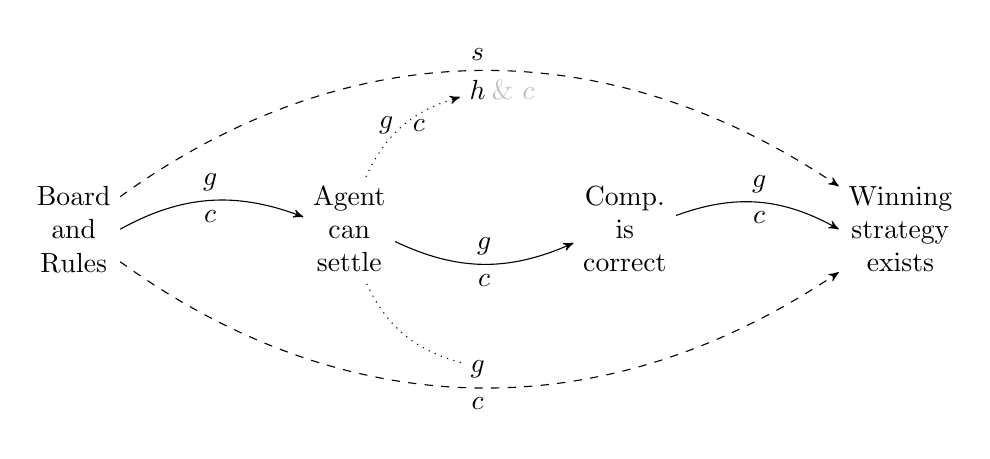
\begin{tikzpicture}[
  ->,
  >=stealth',
  % auto,
  node distance=0cm, every text node part/.style={align=center},
  ]

  \node (1) [] {Board \\ and \\ Rules};
  \node (2) [right of=1, xshift=3.5cm] {Agent \\ can \\ settle};
  \node (3) [right of=2, xshift=3.5cm] {Comp.\ \\ is \\ correct};
  \node (4) [right of=3, xshift=3.5cm] {Winning \\ strategy \\ exists};

  % \draw [->] (1.0) to [bend right=25] (2.180);
  % \draw [->] (2.0) to [bend left=25] (3.180);
  % \draw [->] (3.0) to [bend right=25] (4.180);

  \draw [->] (1.0) to [bend left=25] node[below] {\(c\)} node[above] {\(g\)} (2.165);
  \draw [->] (2.345) to [bend right=25] node[below] {\(c\)} node[above] {\(g\)} (3.195);
  \draw [->] (3.15) to [bend left=25] node[below] {\(c\)} node[above] {\(g\)} (4.180);

  \draw [dashed, ->] (1) to [bend left=35] node[below] (bSH) {\(h\)} node[above] (aSH) {\(s\)} (4);
  \node (x) [right of=bSH, xshift=.45cm, opacity=.25] {\(\&\mbox{ }c\)};
  % \draw [dotted, ->] (1) to [bend left=70] node[below] (bSC) {\(c\)} node[above] {\(s\)} (4);
  \draw [dashed, ->] (1) to [bend right=35] node[below] {\(c\)} node[above] (aGC) {\(g\)} (4);

  \draw [dotted, ->] (2) to [bend left=25] node[right] {\(c\)} node[left] {\(g\)} (bSH);
  % \draw [dotted, ->] (aSH) to [bend right=5] (bSC);
  \draw [dotted, -] (aGC) to [bend left=25] (2);
\end{tikzpicture}
\caption{Main relations}
\label{fig:dynamics}
\end{figure}

\begin{note}
  The general form of the agent's reasoning.
\end{note}

There is some process \(f\) that would yield \(\psi\) from \(\Phi\).
\[
\exists f(f(\Phi) = \psi)
\]

Some process \(g\) uses the existence of a process \(f\) that would yield \(\psi\) from \(\Phi\) and \(\Phi\) to obtain \(\psi\).
\[
  g(\{\exists f(f(\Phi) = \psi), \psi\}) = \psi
\]
The question is whether there is anything to be said about \(g\).
I think there is something to be said, and I will use the term \emph{speculation}.
Broadly stated, \(g\) involves the agent introducing an expression \(\future{f}\) that promises refer to some \(f\) such that \(f(\Phi) = \psi\).
For, if the agent is confident that there exists some \(f\) such that \(f(\Phi) = \psi\) then it is possible for \(\future{f}\) to refer to one such function.
And, given \(\future{f}\) the agent applies \(\future{f}\) to \(\Phi\) to obtain \(\psi\).

\subsection{Application}
\label{sec:application}




\section{Other scenarios}
\label{sec:other-scenarios}

\subsection{Morse}
\label{sec:morse-1}



\begin{scenario}[Morse]
  Morse and Lewis are detectives who are equally matched and have complied a dossier about a case together.
  Morse has some free time, and Lewis is busy.
  Morse leaves a message on Lewis' answering machine stating that Morse has been reviewing the dossier and is confident that Smith is guilty.
  Lewis is confident that the dossier supports the guilt of Smith.
\end{scenario}

\begin{note}
  \begin{itemize}
  \item One of the interesting features of the Morse scenario is that while Lewis forms a promise, it's not clear that Lewis needs to be the one to fulfil the promise.
    It could be that Morse and Lewis have an established relationship, and when Morse informs Lewis that there is a case, Morse is taking on the responsibility of providing a reference to a promised future.
  \item On the other hand, in contrast to the Chess case, the relation to action is much clearer in the Morse case.
  \end{itemize}
\end{note}

More and Lewis, well.
\begin{itemize}
\item Morse can be seen as providing testimony that \(\exists f(f\Phi = \psi)\).
  \begin{itemize}
  \item Is this testimony that \(\psi\)?
  \item Possibly, because Morse has \(\Psi\), and it's would not be possible for Morse to deny \(\psi\) if pressed.
  \item And this isn't how testimony usually works.
  \item Indeed, could make things more complex, assuming that only Lewis has certified some of the evidence.
  \item Hence, Morse may not be in a position to straightforwardly testify that \(\psi\).
  \end{itemize}
\end{itemize}


\subsection{Shopping}
\label{sec:shopping}

\begin{scenario}[Shopping]
  Agent is shopping in a supermarket and has an end.
  On the shopping list is an item.
  The agent cannot immediately recall how the item relates to the end, but is confident that they put the item on the shopping list in service of the end.
  The agent is confident that purchasing the item is worthwhile means to the end, but they are not sure how.
\end{scenario}

\begin{note}
  \begin{itemize}
  \item Here, the key is an additional promise, and a shift in focus.
  \item For, the reasoning from the ends to the means does not seem too difficult, and hence it's specifying the ends which is key.
  \end{itemize}
\end{note}


\subsection{Overview of additional cases}
\label{sec:overv-addit-cases}

In each of the cases the agent has some body of information, and has some additional information which states that some proposition follows from the body of information.
The agent is confident that they could, independently of the additional information, reason from the body of information to the proposition which they have been informed follows.

I am interested in defending the claim that the agent's attitude toward the proposition which follows from the body of information is (in part) based on the body of information.
For, then, these are scenarios in which an agent forms an attitude toward a proposition (in part) on the basis of information they have without reasoning from the information to the adoption of the attitude toward the proposition.

The quick argument for this is that in each of these scenarios the relevance of the additional information which states that some proposition follows from the body of information is relevant only if the agent has the appropriate attitude toward the body of information.
So, as the additional information only states what follows from the body of information, the agent must appeal to the support that the body of information provides for the attitude that they adopt toward the proposition to be supported.
However, as the agent has relied on the additional information in order to recognise that the proposition follows, the agent is not aware of how the body of information supports the proposition.

More detail is required to adequately state what is going on in these situations, but it is plausible that we often find ourselves in situations which have (something sufficiently like) this structure, and understanding these types of situations may help develop our understanding of creatures like us.

A straightforward question is the rational status of agents in situations like these.
For, it seems intuitive that an agent holding an attitude based on a body of information without being aware of how the body of information supports the proposition is not ideally rational.
Unfortunately, I do not think that the relevant structural features are sufficient to support general remarks about the rational status of the agent's in the scenarios if ideal rationality is not required.


\section{Framework}
\label{sec:framework}

Function \(f\) such that this goes from support to proposition.
Familiar idea, e.g.\ logic tells us about when certain functions can be applied.
And, if something like this is right then by generous use of composition there's one big function.

Quite abstract, but this is enough to see the basic idea.
Typically, \(f(\Phi) = \psi\), this is all filled in.
In standard case, \(f\) and \(\Phi\), along with some restrictions on \(f\).

Here, function is capturing some dynamic process.
The types of the proposition may be important.
However, these are a precondition and not an argument of the function.
So, this avoids \citeauthor{Broome:2019aa}'s worries about linking conditions.


Now, in the cases of interest, \(\exists f(f(\Phi) = \psi)\).
So, something like the distinction between reference \emph{de re} and reference \emph{de dicto}.

This doesn't quite capture everything, as there's some additional properties ascribed to everything.

\[\exists f(f(\Phi) = \phi, \delta(f) \cdots)\]

Of course, this is assuming a unique proposition, but perhaps there's a number of permissible propositions, for example if \(f\) is thought of as a consequence relation.
So, here it's simple to compose functions of different types, but this isn't too important.

\begin{itemize}
\item Something about this being relativised to the agent, so \(f\) is not an additional piece of information, as in the case of testimony.
\end{itemize}

So, now

\[g(\{\exists f(f(\Phi) = \phi \land \delta(f) \cdots)\} \cup \Phi) = \phi\]

The \(g\) is whatever happens in the agent's moving from the possibility of reasoning from \(\Phi\) to \(\phi\) and \(\Phi\) to \(\phi\).
Somehow the agent gets a hold of the result of \(f\).

The question is what's happening with this \(g\).
Suggestion is that there's a \emph{promise}.




In \citeauthor{Siegel:2019aa}'s (\citeyear{Siegel:2019aa}) terminology, there is no `reckoning'.
The type of case is related, though distinct.
In the type of cases \citeauthor{Siegel:2019aa} discusses, agent's draw inferences in ignorance of the exact factors that they are responding to (\citeyear[8]{Siegel:2019aa}).
By contrast, in the types of cases under consideration the agent may be aware of the factors that they are responding to, and is aware that an inference to some proposition can be drawn, but is unaware of what the inference is.
Here, then, unclear that the interest is in inference, specifically.
I.e.\ not going to make the claim that the agent infers the relevant proposition \emph{and} it's possible for one to keep hold of the reckoning model that \citeauthor{Siegel:2019aa} argues against while puzzling about these types of cases.


\subsection{Promises}
\label{sec:promises}

\begin{itemize}
\item promise stands in place of some to-be-done process.
\item I promise that when I will understand this, I'll call back.
\end{itemize}

A promise is a proxy for a result that it initially unknown.

\begin{itemize}
\item pending state
\item promises are fulfilled
\item A promise is a container for an as-yet-unknown value
\item extract the value out of the promise and give it to another process
\end{itemize}


This is a more-or-less technical term, especially as in these cases the promise is something that is not shared.
However, there's some intuition, especially when one considers interacting with the agent.

The idea is that the agent makes something like a promise.
They provide something which looks like a function, and this is used to obtain \(\phi\).

Here, with the existential, it's nothing new.
Taking a fresh variable, with the promise that this \emph{can} be given a referent.

\subsection{Smiley}
\label{sec:smiley}

This is similar to how Smiley uses the name `Gregory'.
There's a promise that the name will be given a referent.
This is a useful case to work through, as Smiley builds towards fulfilling the promise.

And, in the clocksmith example, the clock is also a promise, that if the agent were to look at an accurate source of time, things would work out.

\subsection{Logic}
\label{sec:logic}

\begin{note}
  Here I'm only dealing with the reasoning, so there's no discussion of justification and so on.
  All that's happening is an account of the reasoning that's going on in the case of promises.
\end{note}

This about some rules governing existentials.
Standard idea is to take a fresh constant, and show that something follows from this.
The existential guarantees that the term refers, but have no idea what to, and the fresh constant is used with the promise that it is referential.

The principle is similar to existential elimination rules.
Given a formula of the form \(\exists x Px\), fresh constant \(a\) and use this to reason about an object that \(P\) holds of.

% \begin{multicols}{2}
\begin{prooftree}
  \AxiomC{\(\exists x Px\)}
  \AxiomC{}
  \RightLabel{\scriptsize(1)}
  \UnaryInfC{\(Pa\)}
  \AxiomC{\(\forall x(Px \rightarrow Qx)\)}
  \RightLabel{\scriptsize \(\forall\) E}
  \UnaryInfC{\(Pa \rightarrow Qa\)}
  \RightLabel{\scriptsize \(\rightarrow\) E}
  \BinaryInfC{\(Qa\)}
  \RightLabel{\scriptsize \(\exists\) I}
  \UnaryInfC{\(\exists x Qx\)}
  \RightLabel{\scriptsize 1 \(\exists\) E}
  \BinaryInfC{\(\exists x Qx\)}
\end{prooftree}

This can be reformulated.

\begin{prooftree}
  \AxiomC{\(\exists x Px\)}
  \AxiomC{}
  \RightLabel{\scriptsize(1)}
  \UnaryInfC{\(\future{a}\)}
  \BinaryInfC{\(Pa\)}
  \AxiomC{\(\forall x(Px \rightarrow Qx)\)}
  \UnaryInfC{\(P\future{a} \rightarrow Q\future{a}\)}
  \BinaryInfC{\(Q\mathcal{a}\)}
  \UnaryInfC{\(\exists xQx\)}
\end{prooftree}



Quantification over elements is standard, but this can be extended to functions.

\begin{prooftree}
  \AxiomC{\(\exists f(fa = b)\)}
  \AxiomC{}
  \RightLabel{\scriptsize(1)}
  \UnaryInfC{\(\future{f}a = b\)}
  \AxiomC{\(Pb\)}
  \RightLabel{\scriptsize \(=\) E}
  \BinaryInfC{\(P\future{f}a\)}
  \RightLabel{\scriptsize \(\exists\) I}
  \UnaryInfC{\(\exists f Pfa\)}
  \RightLabel{\scriptsize 1 \(\exists\) E}
  \BinaryInfC{\(\exists f Pfa\)}
\end{prooftree}
% \end{multicols}

Here, need to reintroduce quantification over \(f\) because the premises do not provide a way of referring to \(f\).

Straying further from standard proof systems, introduce a function and bind this to the function that is stated to exist.

\begin{prooftree}
  \AxiomC{\(\exists f(fa = b)\)}
  \AxiomC{}
  \RightLabel{\scriptsize(1)}
  \UnaryInfC{\(\future{f}\)}
  \RightLabel{\scriptsize 1 B}
  \BinaryInfC{\(\future{f}a = b\)}
  \AxiomC{\(Pb\)}
  \RightLabel{\scriptsize \(=\) E}
  \BinaryInfC{\(P\future{f}a\)}
  \RightLabel{\scriptsize 1 \(\exists\) E}
  \UnaryInfC{\(\exists fP(fa)\)}
\end{prooftree}

In these examples, \(a\) and \(\future{f}\) are fresh, and \(\psi\) is inferred on the basis of these, and because no assumptions are made regarding \(a\) and \(\future{f}\), one can be sure that \(P\) holds of some transformation of \(a\).

Deductive system, hence the need to discharge assumptions.

Abstracting further, bind function and apply to something.
\(n B\) denotes the binding of the future \(n\).

\begin{prooftree}
  \AxiomC{\(\exists f (f\Phi = \psi)\)}
  \AxiomC{}
  \RightLabel{\scriptsize(1)}
  \UnaryInfC{\(\future{f}\)}
  \RightLabel{\scriptsize 1 B}
  \BinaryInfC{\(\future{f}\Phi = \psi\)}

  \AxiomC{}
  \RightLabel{\scriptsize(1)}
  \UnaryInfC{\(\future{f}\)}
  \AxiomC{\(\Phi\)}
  \RightLabel{\scriptsize 1 A}
  \BinaryInfC{\(\future{f}\Phi\)}

  \RightLabel{\scriptsize \(=\) E}
  \BinaryInfC{\(\psi\)}
  % \RightLabel{\scriptsize 1 \(\exists\) E}
  % \UnaryInfC{\(\psi\)}
\end{prooftree}

The idea remains the same, use the guarantee of reference to reason with a specific instance with a referring term.
As before, obtain \(\psi\), for if \(\Phi\) holds, and there is some transformation of \(\Phi\) which yields \(\psi\) then \(\psi\) holds.
\begin{note}
  Think about Skolemization.
\end{note}

The difficulty for the agents in the scenarios is the existential statement, and whether this is in fact true.

\subsection{Scenarios}
\label{sec:scenarios-1}

The key promise in each of the scenarios is a process, but there are additional things involved.
For, in the chess there's a question of what the strategy is, and in the supermarket what the agent's ends are.
Morse, then, is the simplest case from this point of view.
Chess is particularly interesting, then, as the agent doesn't know exactly what the fulfilment of the promise would result in.
And, Supermarket is interesting because the agent isn't sure of what the preconditions of the promise are.
However, in order for the promise to be fulfilled the agent only needs to be sure that the preconditions can be met.

\begin{itemize}
\item Chess: guarantee of something with a particular property given by some process
\item Morse: guarantee of a demonstration
\item Supermarket: guarantee (primarily) of attitudes.
\end{itemize}



The scenarios abuse promises, because the agent is confident about what the promise returns.
Usually one needs to be led to the table.
The situation is similar to looking in the window of the restaurant, identifying a table without a reservation, calling to make the reservation, and then walking in and sitting down at the table.
In a wild breach of protocol I am not led to the table, but I'm sufficiently confident that I am sat at the table that I would be led to were I to be led.


The chess scenario is the clearest case.
Here, the agent must make a promise in order to form the relevant attitude toward the existence of a winning strategy.
That is, the agent's confidence that they can reason promises that there is some process that the agent can perform.

\subsubsection{Morse}
\label{sec:morse}



The Morse scenario is less clear.
It's not straightforward that Lewis needs to make a promise.
However, if Lewis forms the belief that Smith is guilty, then there's a promise that needs to be fulfilled, and it either falls on Lewis or Morse.
However, this is about fulfilment of the promise.
To the extent that Lewis accepts the promise, there's a direct route from the evidence to Lewis' belief.


In the examples, the distinguishing feature is that the agent has what they would want from a fulfilment of the promise.
The promise is that this is how things would work out.

This neatly illustrates what's going on between the superman and tax examples.
For, in the superman case the agent's failure to draw the obvious inference suggests that the agent cannot keep the promise.
While, in the tax example it is quite plausible that the agent can keep their promise.

So, because the promise is about what the agent can do, there's no appeal to additional information.

\begin{itemize}
\item Making use of the idea of a contract might be nice here, as plausibly it's the case that Lewis cannot establish a contract with Morse, wherein Morse would guarantee to fulfil the promise.
\item Or, maybe Lewis can.
\item This is something intuitions will with.
\end{itemize}

\subsubsection{Supermarket}
\label{sec:supermarket}


\begin{prooftree}
  \AxiomC{\(\exists f \exists X(fX = \psi)\)}
  \AxiomC{}
  \RightLabel{\scriptsize(1)}
  \UnaryInfC{\(\future{f}\)}
  \RightLabel{\scriptsize 1 B}
  \BinaryInfC{\(\future{f}X = \psi\)}
  \AxiomC{}
  \RightLabel{\scriptsize (2)}
  \UnaryInfC{\(\future{X}\)}
  \RightLabel{\scriptsize 2 B}
  \BinaryInfC{\(\future{f}\future{X} = \psi\)}

  \AxiomC{}
  \RightLabel{\scriptsize(1)}
  \UnaryInfC{\(\future{f}\)}
  \AxiomC{}
  \RightLabel{\scriptsize (2)}
  \UnaryInfC{\(\future{X}\)}
  \RightLabel{\scriptsize 1 2 FA}
  \BinaryInfC{\(\future{f}\future{X}\)}

  \RightLabel{\scriptsize \(=\) E}
  \BinaryInfC{\(\psi\)}
\end{prooftree}


\subsection{Speculation}
\label{sec:speculation}

\emph{This} is what's going on.
In each of the cases the process has a predictable result, and the agent continues based on this.
If the agent's speculation is correct, then a whole bunch of effort is saved.
If the agent's speculation is not correct, then the agent has a problem, and needs to do some work.

\subsection{Notes}
\label{sec:notes}

\begin{note}
  This is the cheaters defence.
  The cheater promises that they could have reasoned.
\end{note}

\begin{note}
  Things get more interesting when there's a sort of pipeline, and the agent can choose between using what's at the end of the pipeline or waiting for something fresh.
\end{note}

\subsection{Similar kind of scenario}
\label{sec:simil-kind-scen}

\begin{scenario}[Clocksmith]
  In the hallway between classes is an old clock.
  As the clock is old it has a tendency to be inaccurate.
  The agent is aware that a clocksmith comes by every now and again to correct the clock.
  The agent is also aware that the clocksmith does so by setting the clock to the same time as the clocksmith's digital watch.
  The agent exits a class and sees the clocksmith walking away, looks at the clock, and forms the belief that it's three thirty.
  The agent's belief is not based on the clock accurately displaying three thirty as the time, but on the clocksmith having an accurate digital watch and that the clock has been recently serviced to display the same time as the time on the clocksmith's digital watch.
\end{scenario}

Here, the agent does not have a body of information with which to determine the time, but similar to the previous scenarios the clock is providing information about what a distinct body of information supports, namely what the clocksmith's digital watch states the time as.

\section{Constructive and non-constructive support}
\label{sec:constr-non-constr}

Intuitive idea is that the additional body of information provides non-constructive support for the proposition, and the agent reasoning from the body of information would provide constructive support.

For, in each of the cases the agent is confident that the proposition follows from the body of information that they have given reasoning that the agent is able to do.
Hence, the agent does not need any additional information or further capabilities as a reasoner to show that the body of information supports the proposition.

The distinction between constructive and non-constructive support rests on the idea that bodies of information stands in structural relations to other propositions.
Constructive support shows the structural relations between the body of information and relevant proposition, while non-constructive support establishes that some relation exists.

% Structure comes from the Latin \emph{struere} `to build'
% Constructive comes from the Latin \emph{constructuere}, from \emph{con-} `together' + \emph{relation} `to build' (i.e. the bringing together of objects to build).

The distinction between constructive and non-constructive support is similar to the idea of a constructive proof in logic/mathematics.
In the chess scenario there are clear parallels to the idea of a constructive proof.
For, in the chess scenario the agent is confident that a winning strategy exists, but is unable to provide a witnessing strategy.
And, were the agent to reason from the state of the board and the rules of chess the agent would be able to provide a witnessing strategy.
However, in the Morse and shopping scenarios the relevant proposition contains neither an existential nor a disjunction.
In the Morse scenario Lewis is confident that the individual Smith is guilty, and in the shopping scenario the agent is confident that it is worthwhile to purchase a particular item.
Therefore, it is difficult to cast these scenario in terms of providing a witness for the supported proposition.
Yet, similar to constructive implication, where \(A \rightarrow B\) requires demonstrating how to construct \(B\) from \(A\).

\begin{note}
  I think something a long these line is the right thing to focus on.
  It's possible to appeal to distinct rational pressures, correctly responding to reasons, some notion of understanding, and so on, but each of these idea brings in additional commitments that aren't necessarily required to state the phenomena, and may be best left as resources for supporting judgements about the scenarios.

  Understanding, in particular, is interesting as it's not clear that there's a variation on the Morse scenario where Lewis does not understand why Smith is guilty, but would understand how the evidence supports the guilt of Smith.
  For example, Smith may be involved in some kind of financial fraud and the dossier lists a number of statutes which linked together based on formal features implicate Smith.
  And, Lewis may be able to piece together the formal features of the statues, but have no idea what these ensure Smith is guilty of.
\end{note}

\subsection{D.E.\ Over}
\label{sec:d.e.-over}

I've been reading through a collection of papers by \citeauthor{Over:1983ab} who discusses some connexions between knowledge, reasoning, and constructive mathematics.
Unfortunately these papers are quite old, weren't discussed, and tie constructive knowledge/reasoning to being able to provide the reference of a proposition (which is difficult to extend to the cases I'm interested in, as it seems to me the issue I'm dealing with is providing the support for a proposition).
Still, of note is that \citeauthor{Over:1983ab} describes a very similar scenario to what I've been thinking about.

\begin{quote}
  \begin{enumerate}[label=(\arabic*)]
    \setcounter{enumi}{8}
  \item Someone in the identity parade murdered Bexley.
  \end{enumerate}

  \mbox{}\hfill\vdots\hfill\mbox{}

  Suppose, however, that the police have constructive knowledge that (9) is true.
  They may be able to pick out the murderer straightaway; and they would then certainly have predicative or \emph{de re} knowledge.
  They must at least have a procedure that leads to the murderer in a finite time, such as checking the finger prints of all the suspects in the parade.
  Again, they certainly have predicative knowledge if they have followed the procedure to its end and pointed out the guilty party.
  But suppose they have the procedure but do not follow it?
  They know that the murderer is in the identity parade, that they have his finger prints, and that they could, with a little trouble, separate him from the rest; but for some reason they do not do this.
  Do they have predicative knowledge that (9) is true?
  That is, do they know of someone in the identity parade, that he murdered Bexley?
  It does seem natural to say that they do, although this may involve some extension of our admittedly vague understanding of predicative knowledge.
  The police in this case are in a much stronger position than someone who simply has \emph{de dicto} or propositional knowledge that (9) is true; the police are much closer to central cases of predicative or \emph{de re} knowledge.\nolinebreak
  \mbox{}\hfill\mbox{(\citeyear[143--144]{Over:1983ab})}
\end{quote}

Unfortunately, \citeauthor{Over:1983ab} does not discuss the case in greater detail, nor does \citeauthor{Over:1983ab} discuss a similar case in any of the connected papers I have looked through (\citeyear{Millican:1990aa,Over:1987aa,Over:1986aa,Over:1985aa,Over:1983ab,Over:1983aa}).
And, as mentioned above, \citeauthor{Over:1983ab}'s interest in connecting constructive knowledge/reasoning to the \emph{de re}/\emph{de dicto} distinction makes linking \citeauthor{Over:1983ab}'s discussion to my scenarios difficult.

\section{No general lessons about rationality}
\label{sec:no-general-lessons}

Present two scenarios which have the same structure as the main scenarios, but where intuitions about rationality conflict.

\begin{scenario}[Superman]
  Agent is tasked with purchasing shoes for Superman, and is confident that Superman has size 11 feet.
  The agent is also confident that superman is Clark Kent is Superman.
  The agent mentions these two beliefs to a companion, and the companion remarks that although they assumed that Clark Kent had size 13 feet, it follows from what the agent has said that Clark Kent has size 11 feet.
  The agent, on the basis of the companion pointing out that Clark Kent having size 11 feet follows from the belief that the agent has, forms the belief that Clark Kent has size 11 feet.
\end{scenario}

I suspect that agent in the superman scenario cannot be interpreted as a rational agent.
For, it seems as though it should be clear to the agent that from their belief that Clark Kent is Superman and their belief that Superman has size 11 feet that Clark Kent has size 11 feet.

\begin{scenario}[Calculator]
  Agent is filing taxes, and needs to know the result of multiplying two numbers.
  The multiplication is not hard, and the agent is a competent mathematician.
  However, not wishing to spend more time than necessary on their taxes, the agent asks a companion what the result of the multiplication is, and writes in the companions answer.
\end{scenario}

It seems hard to fault the agent in this case, even though multiplying the two numbers may be no less obvious than substituting Clark Kent for Superman in the contrasting case.
The agent has some body of information, that two numbers multiplied would give a required value and a background grasp of mathematics, and is capable of determining the required value without any additional information, but relies on a companion informing them of what the required value is.

\subsection{Notes on ideal rationality}
\label{sec:notes-ideal-rati}

It seems intuitive that an ideal agent would not rely on non-constructive support for any given proposition that they hold an attitude toward.
For, without limitations there is no barrier to the ideal agent establishing constructive support for the proposition.

This argument may be a little too quick, however.
For, if it is possible for an ideal agent to have a body of evidence without yet having constructive support for the propositions supported by that body of evidence, then scenarios may be constructed which prevent the agent from obtaining anything but non-constructive support.

\begin{scenario}[Secrets]
  Suppose we have an ideal agent and a non-companion who are on a mission together.
  The agent and companion have been given a dossier, and some reasoning is required to extract a password to a door from the dossier.
  The companion has extracted the password by some reasoning, but before the agent is able to extract the password they discover that some non-capable adversary is able to read their mind.
  Hence, if the ideal agent reasons to the password the non-ideal adversary will have access to the password, but if the ideal agent does not reason to the password there is a good chance that the non-ideal adversary will not discover what the password is.
  However, just as the adversary is non-ideal, the ideal agent's companion is also non-ideal, and the ideal agent would like to be arbitrarily confident that the non-ideal companion has successfully extracted the password.
  Luckily, a backup plan has been prepared.
  [The cave example again, noting also that the adversary can't be sure that the agent and companion hadn't prepared the sequence in advance.]
\end{scenario}


\section{Siegel}
\label{sec:siegel}

\citeauthor{Siegel:2019aa} notes that if inference meets \citeauthor{Boghossian:2014aa}'s self-awareness condition, `then inferrers are never ignorant of the fact that they are responding to some of their psychological states, or why they are so responding.' (\citeyear[6]{Siegel:2019aa})

\begin{description}[font=\bfseries, leftmargin=.75cm, style=nextline]
\item[Self-awareness condition] Person-level reasoning [is] mental action that a person performs, in which he is either aware, or can become aware, of why he is moving from some beliefs to others.\nolinebreak
  \mbox{}\hfill\mbox{(\citeyear[16]{Boghossian:2014aa})}
\end{description}





`Sometimes when one categorizes what one perceives, one is not aware of which features lead one to categorize as one does.' \citeyear[9]{Siegel:2019aa}

\begin{scenario}[Kindness]
  The person ahead of you in line at the Post Office is finding out from the clerk about the costs of sending a package. Their exchange of information is interspersed with comments about recent changes in the postal service and the most popular stamps. As you listen you are struck with the thought that the clerk is kind. You could not identify what it is about the clerk that leads you to his thought. Nor could you identify any generalizations that link these cues to kindness. Though you don’t know it, you are responding to a combination of what she says to the customer, her forthright and friendly manner, her facial expressions, her tone of voice, and the way she handles the packages.\nolinebreak
  \mbox{}\hfill\mbox{(\citeyear[9--10]{Siegel:2019aa})}
\end{scenario}


\begin{scenario}[Pepperoni]
  Usually you eat three slices of pizza when it comes with pepperoni.
  But tonight, after eating one slice, you suddenly don't want any more.
  Struck by your own uncharacteristic aversion, you form the belief that the pizza is yucky.
  Though you don't know it, you’re responding to the facts that
  \begin{enumerate*}[label=(\roman*)]
  \item the pepperoni tastes very salty to you,
  \item it looks greasy,
  \item it reminds you of someone you don’t like, who you recently learned loves pepperoni, and
  \item you have suddenly felt the force of moral arguments against eating meat.
  \end{enumerate*}
  If the next bites of pepperoni were less salty, the greasy appearance turned out to be glare from the lights, you learned that your nemesis now avoids pepperoni, and the moral arguments didn't move you, the conclusion of your inference would weaken, and so would your aversion.
  You haven't classified what you see and taste as: too greasy, too salty, reminiscent of your nemesis, or the sad product of immoral practices.
  Nor are you consciously thinking right now about any of these things.\nolinebreak
  \mbox{}\hfill\mbox{(\citeyear[11]{Siegel:2019aa})}
\end{scenario}

\section{Connexions to the literature}
\label{sec:conn-liter}

\subsection{Buchak}
\label{sec:buchak}

\textcite{Buchak:2014aa} discusses ``the problem of naked statistical evidence'' in the context of the case of the green and yellow buses and argues that belief cannot be reduced to credence.

I'm inclined to think, possibly due to this being suggested to me, that there's no need to frame my cases in terms of statistical evidence, and instead see statistical evidence as a way of generating non-constructive support for a proposition.
However, to the extent that it is possible to construct cases involving statistical evidence, then \citeauthor{Buchak:2014aa}'s argument that belief and credence are distinct offers a way to understand the different kind of support available to the agent, and \citeauthor{Buchak:2014aa}'s discussion of the norms associated with blame may provide some explanation of judgements about (as subset of) the kind of cases I've been thinking of.

So, at the very least, \citeauthor{Buchak:2014aa}'s paper is an additional connexion to broader literature, and there is the possibility of generalising some of \citeauthor{Buchak:2014aa}'s discussion.

\subsection{Fogal}
\label{sec:fogal}

So, I see the role of promises as relating to structural rationality, in a way.
However, I don't think that there's necessarily an immediate application of structural rationality.
For, I think the agent's promise is important.
So, it's slightly different.

\subsection{Lord}
\label{sec:lord}

\citeauthor{Lord:2018aa} is of interest because the agent is likely irrational, given \citeauthor{Lord:2018aa}'s account.
The argument is a little more subtle though, as there is some wiggle room, for perhaps there is a appropriate notion of correctly responding.
The difficulty is specifying what this is while maintaining a distinction between the types of cases that I have in mind.

\section{Related cases}
\label{sec:related-cases}

These involve Rosamund, a liberal arts education, and so on.
In these cases, the agent has the ability, but does not make a promise.
May think that this is a problem, but it is slightly different, as the agent does not make a claim, and if there is some pressure, this pressure is independent.


\newpage

\printbibliography

\end{document}
